\chapter{Komunikace s platformou}
\label{sec:PlatformCommunication}
\vspace{-20pt}
\

Během jízdy komunikace s platformou bylo implementováno na základě \textbf{UDP}
(User Datagram Protocol).  UDP je komunikační protokol,
který se primárně používá pro časové citlivé informace.
Zrychluje komunikaci tím, že před přenosem dat není nutné formálně navazovat spojení.
To umožňuje velmi rychlý přenos dat\cite{UDP}.

Během komunikace vývojová deska se chová jako UDP server a aplikace pro zobrazení dat
je client. Aplikace pro zobrazení dat je \textbf{CarQt} a zobrazuje data z kamery
ve 2D formátu  s~historii záznamu. Zobrazuje originální,
normalizovány a prahový obraz. Další data
jsou zobrazeny v číselném formátu. To jsou informace o regionu, PWM motoru, servo motoru
a senzoru. Zápis číselných dat je implementováno ve formátu \textbf{JSON}
(JavaScript Object Notation) a originálního obrazu ve formátu \textbf{PNG}
(Portable Network Graphics) souboru. CarQt bylo vytvořeno pomocí knihoven Qt a OpenCV.
Aplikace je zobrazena na obrázku \ref{fig:CarQt}
\begin{figure}[!h]
    \centering
    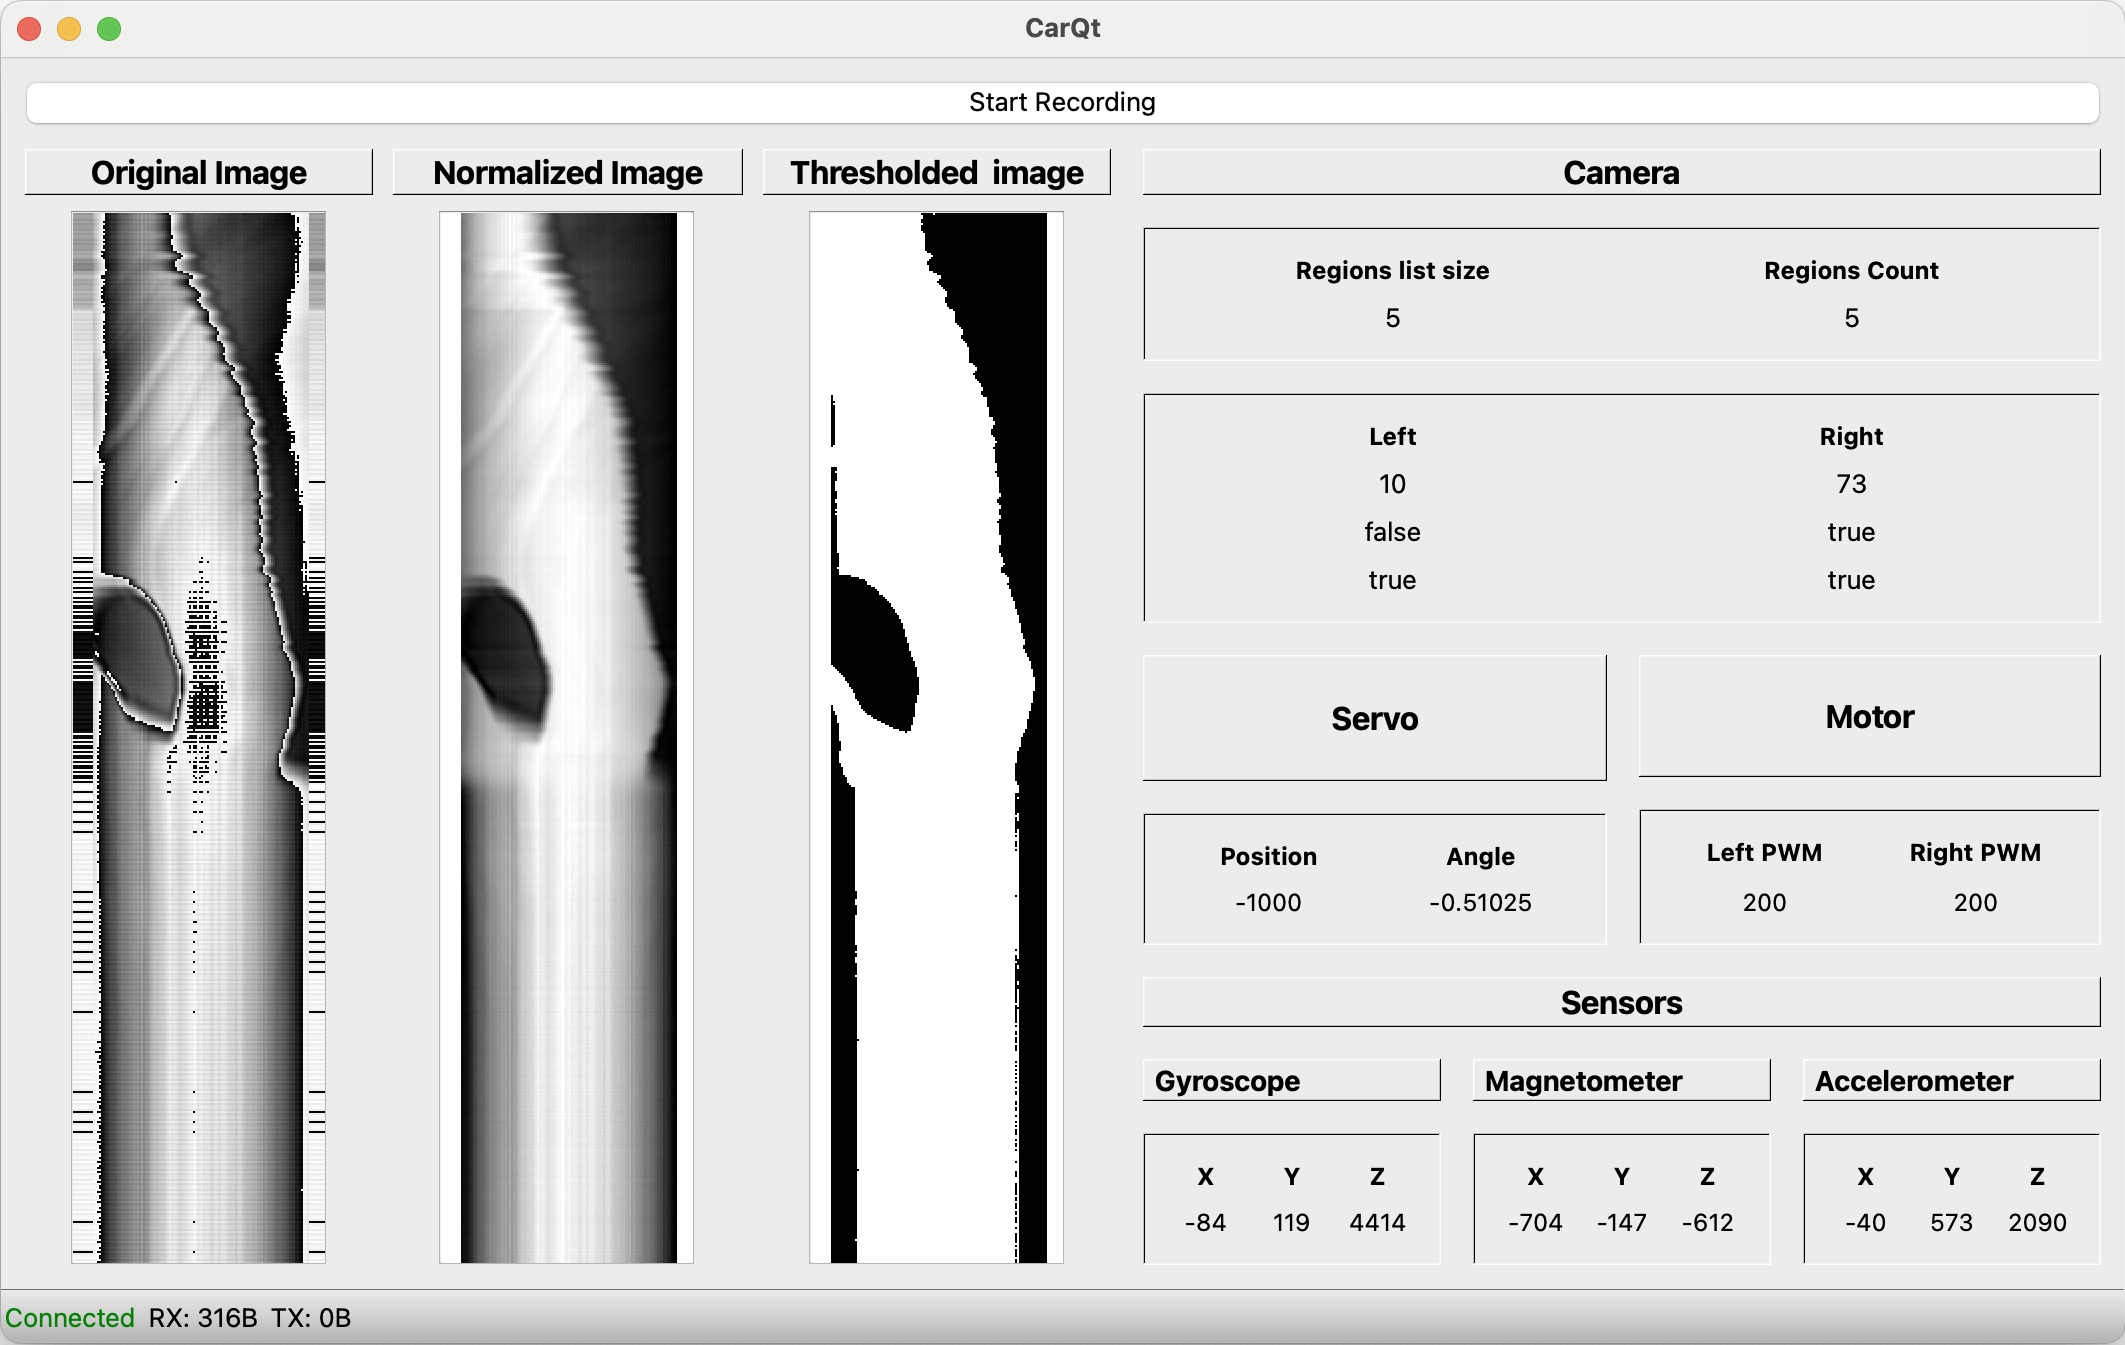
\includegraphics[width = .5\linewidth]{Figures/CarQt.png}
    \caption{CarQt aplikace}
    \label{fig:CarQt}
\end{figure}


Pro přenos data se použita struktura \textbf{Data}, která obsahuje originální data z kamery, regiony, PWM motoru, servo motoru a senzoru. Výpis je \ref{lst:data}
\begin{lstlisting}[caption=structura Data, label=lst:data]
// Data.h
struct Data {
    // Camera data
    uint16_t line[Image::LINE_LENGTH] = {0};
    uint32_t regionsCount = 0;
    uint32_t regionsListSize = 0;
    bool unchangedLeft = false;
    bool unchangedRight = false;
    bool hasLeft = false;
    bool hasRight = false;
    uint8_t leftDistance = 0;
    uint8_t rightDistance = 0;

    // Motor data
    int32_t leftSpeed = 0;
    int32_t rightSpeed = 0;

    // Servo data
    int32_t servoPosition = 0;
    float angle = .0f;

    Vec3<int16_t> accel = {0, 0, 0};
    Vec3<int16_t> mag = {0, 0, 0};
    Vec3<int16_t> gyro = {0, 0, 0};

    uint32_t timestamp = 0;
    uint8_t mode = Mode::None;
};
\end{lstlisting}

\endinput
